% ============================================================
% Lecture 5 -- Basics of Linear Models
% ============================================================
\section{Basics of Linear Models}\label{sec:L05}

\lectureheader{5}{Ec94oyf3bKw}{Week-2 slides \texttt{Feb2.pdf} (``Linear Models'' slides on the \texttt{sim1} data), with annotations; Week-2 R code}

\begin{guiding*}
By the end of this lecture you should be able to:
\begin{itemize}
  \item describe a family of linear models $y=a_1+a_2x$ and the residuals of each member;
  \item explain why the \emph{sum of squared} residuals is the criterion used to choose the best line;
  \item find the best line numerically (\texttt{optim}) and with \texttt{lm};
  \item derive the least-squares estimates $\hat a_2=S_{xy}/S_{xx}$, $\hat a_1=\bar y-\hat a_2\bar x$.
\end{itemize}
\end{guiding*}

\subsection{Recap and motivation}
In \cref{sec:L04} we set ourselves the goal of finding $a_1,a_2$ such that $y\approx a_1+a_2x$.
To see how this works, the instructor uses a simulated data set in which we know there is a
linear pattern: \texttt{sim1}, from the R package \texttt{modelr}.

\subsection{A family of lines}
\begin{example}[The \texttt{sim1} data]\label{ex:L05-sim1}
\texttt{sim1} has $n=30$ points: three $y$-values at each of $x=1,2,\dots,10$. The scatter plot
shows a clear pattern: a linear relationship. To explore possible models, the instructor
generates $250$ lines $y=a_1+a_2x$, with the intercept $a_1$ chosen uniformly from $[-20,40]$ and
the slope $a_2$ uniformly from $[-5,5]$, and plots all $250$ lines on top of the data
(\cref{fig:L05-sim1}, left). Most of them are terrible. A few pass through the cloud of points.
\end{example}

To say which lines are good, we need a number that measures how far a line is from the data.
\begin{definition}[Residual]\label{def:L05-residual}
For the model $y=a_1+a_2x$ and the data point $(x_i,y_i)$, the \vocab{residual} is
\[
e_i(a_1,a_2)=y_i-(a_1+a_2x_i),
\]
the vertical distance (with sign) between the data point and the line. It is the part of $y_i$
that the model does not explain.
\end{definition}

The slides then choose one line from the $250$ (line number $130$), plot it, and draw the
residuals as vertical segments from each point to the line. A good line should make the
residuals small \emph{overall}. The instructor's annotation lists candidate criteria:
\begin{enumerate}
  \item minimise the sum of distances $\sum_i \abs{e_i}$ (``hard'', since $\abs{\cdot}$ is not differentiable);
  \item minimise the sum of squared distances $\sum_i e_i^2$: the \vocab{least squares} criterion (ticked on the slide).
\end{enumerate}

\begin{definition}[Least squares line]\label{def:L05-LS}
For data $\{(x_i,y_i)\}_{i=1}^n$ let
\[
f(a_1,a_2)=\sum_{i=1}^n \bigl(y_i-a_1-a_2x_i\bigr)^2 .
\]
A pair $(\hat a_1,\hat a_2)$ minimising $f$ gives the \vocab{least squares line}
$y=\hat a_1+\hat a_2 x$.
\end{definition}

\subsection{Finding the best line numerically}
The R code on the slides defines the model and a distance, then minimises the distance with a
general-purpose optimiser:
\begin{center}
\begin{minipage}{0.8\textwidth}\small\ttfamily
model1 <- function(a, data) \{ a[1] + data\$x * a[2] \}\\
measure\_distance <- function(mod, data) \{\\
\quad diff <- data\$y - model1(mod, data)\\
\quad sqrt(mean(diff\textasciicircum 2)) \}\\
best <- optim(c(0, 0), measure\_distance, data = sim1)\\
best\$par \qquad\qquad \# 4.222248 2.051204\\
measure\_distance(best\$par, sim1) \# 2.128181
\end{minipage}
\end{center}
The distance used is the \vocab{root mean squared error}
$\mathrm{RMSE}(a_1,a_2)=\sqrt{\tfrac1n\sum_i e_i(a_1,a_2)^2}=\sqrt{f(a_1,a_2)/n}$. The map
$t\mapsto\sqrt{t/n}$ is strictly increasing, so minimising RMSE is the same as minimising $f$.
\texttt{optim} (Nelder--Mead) returns intercept $4.222248$ and slope $2.051204$, with
RMSE $2.128181$. The slide plots this line: intercept $\approx 4.22$, slope $\approx 2.05$. It
seems to give a good approximation.

The slide then asks: \emph{how do we judge the model, and is this the best possible solution?}
The ``to do'' written on the slide is to minimise $f(a_1,a_2)$ exactly. R's built-in function
\texttt{lm(y \textasciitilde\ x, data = sim1)} does this and returns
\[
\hat a_1 = 4.220822,\qquad \hat a_2=2.051533 .
\]
The small difference from \texttt{optim} is numerical: Nelder--Mead stops once further progress
falls below its tolerance. \texttt{lm} solves the problem exactly, as we now show.

\subsection{The least-squares estimates}
\begin{theorem}[Least squares for a straight line]\label{thm:L05-slr}
Let $n\ge 2$ and suppose the $x_i$ are not all equal. Write
\[
\bar x=\tfrac1n\sum x_i,\quad \bar y=\tfrac1n\sum y_i,\quad
S_{xx}=\sum_{i}(x_i-\bar x)^2,\quad S_{xy}=\sum_i (x_i-\bar x)(y_i-\bar y).
\]
Then $f(a_1,a_2)=\sum(y_i-a_1-a_2x_i)^2$ has a unique minimiser
\[
\hat a_2=\frac{S_{xy}}{S_{xx}},\qquad \hat a_1=\bar y-\hat a_2\,\bar x ,
\]
and the minimum value is $f(\hat a_1,\hat a_2)=S_{yy}-S_{xy}^2/S_{xx}$, where $S_{yy}=\sum(y_i-\bar y)^2$.
\end{theorem}
\begin{proof}
We complete the square twice, so that no calculus is needed. For fixed $a_2$ write
$z_i=y_i-a_2x_i$. Then $f=\sum_i(z_i-a_1)^2$. By \cref{prop:L01-bestconst},
\[
\sum_i (z_i-a_1)^2=\sum_i (z_i-\bar z)^2+n(\bar z-a_1)^2,\qquad \bar z=\bar y-a_2\bar x .
\]
Now $z_i-\bar z=(y_i-\bar y)-a_2(x_i-\bar x)$, so
\[
\sum_i (z_i-\bar z)^2=S_{yy}-2a_2S_{xy}+a_2^2S_{xx}
= S_{xx}\Bigl(a_2-\frac{S_{xy}}{S_{xx}}\Bigr)^2 + S_{yy}-\frac{S_{xy}^2}{S_{xx}} ,
\]
where we used $S_{xx}>0$ (the $x_i$ are not all equal). Altogether
\[
f(a_1,a_2)= S_{yy}-\frac{S_{xy}^2}{S_{xx}} + S_{xx}\Bigl(a_2-\frac{S_{xy}}{S_{xx}}\Bigr)^2 + n\bigl(\bar y-a_2\bar x-a_1\bigr)^2 .
\]
The last two terms are non-negative. Both vanish if and only if $a_2=S_{xy}/S_{xx}$ and
$a_1=\bar y-a_2\bar x$. Hence this pair is the unique minimiser, and the minimum is
$S_{yy}-S_{xy}^2/S_{xx}$.
\end{proof}

\begin{corollary}\label{cor:L05-props}
The least-squares line passes through $(\bar x,\bar y)$. The residuals
$\hat e_i=y_i-\hat a_1-\hat a_2x_i$ satisfy $\sum_i\hat e_i=0$ and $\sum_i x_i\hat e_i=0$.
\end{corollary}
\begin{proof}
At $x=\bar x$ the line gives $\hat a_1+\hat a_2\bar x=\bar y$. Next,
$\hat e_i=(y_i-\bar y)-\hat a_2(x_i-\bar x)$. Summing gives $0-0=0$. Also
$\sum_i (x_i-\bar x)\hat e_i=S_{xy}-\hat a_2S_{xx}=0$. Since $\sum\hat e_i=0$, it follows that
$\sum x_i\hat e_i=\sum(x_i-\bar x)\hat e_i+\bar x\sum\hat e_i=0$.
\end{proof}
The two identities $\sum\hat e_i=0$ and $\sum x_i\hat e_i=0$ are exactly the \emph{normal
equations} of \cref{sec:L12}, written out for a straight line.

\begin{example}[A least-squares line by hand]\label{ex:L05-hand}
Take $n=4$ points with $x=(1,2,3,4)$ and $y=(2,3,5,6)$.
\begin{itemize}
  \item $\bar x=2.5$ and $\bar y=16/4=4$.
  \item Deviations: $x_i-\bar x=(-1.5,-0.5,0.5,1.5)$ and $y_i-\bar y=(-2,-1,1,2)$.
  \item $S_{xx}=2.25+0.25+0.25+2.25=5$ and $S_{xy}=3+0.5+0.5+3=7$. Also $S_{yy}=4+1+1+4=10$.
  \item $\hat a_2=7/5=1.4$ and $\hat a_1=4-1.4\times 2.5=0.5$.
  \item Fitted values: $0.5+1.4x=(1.9,3.3,4.7,6.1)$. Residuals: $(0.1,-0.3,0.3,-0.1)$. They sum to $0$, and $\sum x_i\hat e_i=0.1-0.6+0.9-0.4=0$.
  \item Minimum: $f=0.01+0.09+0.09+0.01=0.2$, which agrees with $S_{yy}-S_{xy}^2/S_{xx}=10-49/5=0.2$. The RMSE is $\sqrt{0.2/4}=0.2236$.
\end{itemize}
\end{example}

\begin{figure}[ht]
\centering
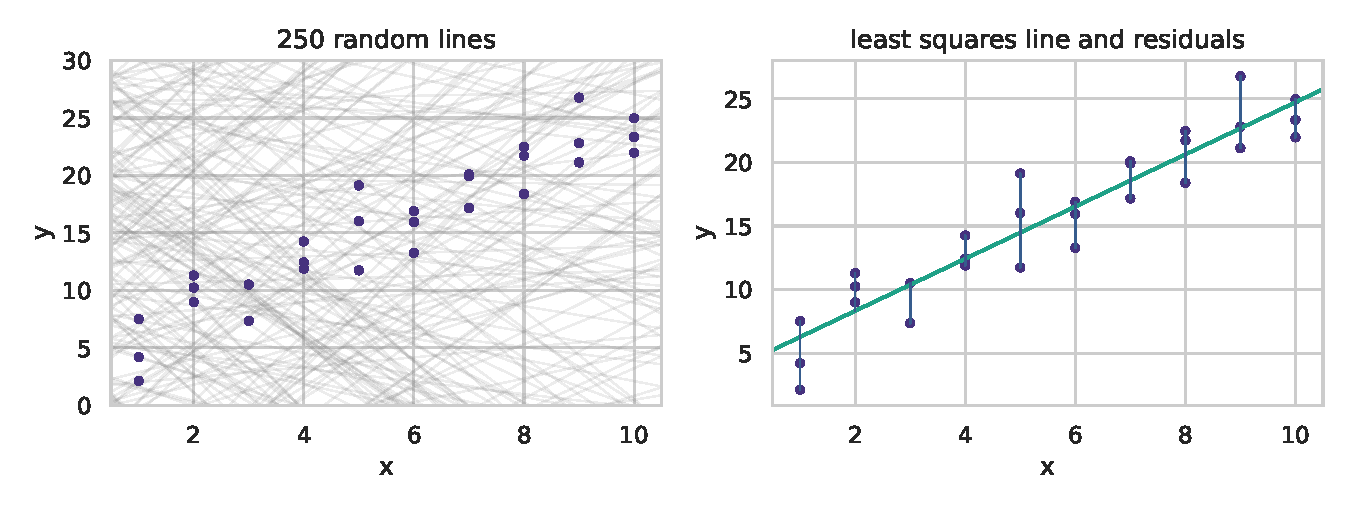
\includegraphics[width=0.95\textwidth]{figures/L05_sim1.pdf}
\caption{Left: $250$ random lines over the \texttt{sim1} data. Right: the least-squares line and its residuals.}
\label{fig:L05-sim1}
\end{figure}

\begin{note}[Supplementary: why squares?]
Squares make $f$ a smooth, convex quadratic, so the minimiser has the closed form of
\cref{thm:L05-slr}. The absolute-value criterion has no closed form and may have many
minimisers. Squares also lead to the Pythagorean geometry of \cref{sec:L12,sec:L14}. Under
normal errors, least squares coincides with maximum likelihood, and the Gauss--Markov theorem
(Week~6) shows that it is optimal among linear unbiased estimators. The price is sensitivity to
outliers: one large residual counts quadratically.
\end{note}

\subsection{Computation}
\begin{center}\small
\begin{tabular}{@{}>{\raggedright\arraybackslash}p{7cm}>{\raggedright\arraybackslash}p{8.4cm}@{}}\hline
R & Python\\\hline
\texttt{runif(250,-20,40)}, \texttt{runif(250,-5,5)} & \texttt{rng.uniform(-20, 40, 250)}, \texttt{rng.uniform(-5, 5, 250)}\\
\texttt{optim(c(0,0), measure\_distance, data=sim1)} & \texttt{scipy.optimize.minimize(rmse, [0,0], method="Nelder-Mead")}\\
\texttt{lm(y \textasciitilde\ x, data=sim1)} & \texttt{smf.ols("y \textasciitilde\ x", data=sim1).fit().params}\\\hline
\end{tabular}
\end{center}
The notebook \nb{week02/L05\_basics\_linear\_models.ipynb} also computes $\hat a_1,\hat a_2$ from
the formulas of \cref{thm:L05-slr} and checks them against \texttt{statsmodels}.

\subsection{Summary}
\begin{itemize}
  \item Residual $e_i=y_i-(a_1+a_2x_i)$. Criterion: minimise $f(a_1,a_2)=\sum e_i^2$ (least squares). This is equivalent to minimising RMSE.
  \item $\hat a_2=S_{xy}/S_{xx}$, $\hat a_1=\bar y-\hat a_2\bar x$, and $\min f=S_{yy}-S_{xy}^2/S_{xx}$.
  \item The fitted line passes through $(\bar x,\bar y)$, and $\sum\hat e_i=\sum x_i\hat e_i=0$.
  \item \texttt{sim1}: \texttt{lm} gives $4.220822$ and $2.051533$ (RMSE $2.128181$). \texttt{optim} agrees to about three decimals.
\end{itemize}

\subsection{Exercises}
\begin{problem}\label{prob:L05-1}
Show that $S_{xy}=\sum_i (x_i-\bar x)y_i=\sum_i x_iy_i-n\bar x\bar y$.
\end{problem}
\begin{problem}\label{prob:L05-2}
Fit the least-squares line by hand to $x=(0,1,2)$, $y=(1,1,4)$. Give the residuals and the minimum of $f$.
\end{problem}
\begin{problem}\label{prob:L05-3}
Show that if we fit the line through the origin, $y=a_2x$, the least-squares slope is $\sum x_iy_i/\sum x_i^2$.
\end{problem}
\begin{problem}\label{prob:L05-4}
What happens in \cref{thm:L05-slr} if all $x_i$ are equal? Describe the set of minimisers.
\end{problem}
\begin{problem}\label{prob:L05-5}
Minimise $\sum\abs{e_i}$ for \texttt{sim1} numerically (Nelder--Mead) and compare the line with the least-squares line.
\end{problem}

\subsection{Further reading}
Wickham \& Grolemund, \emph{R for Data Science}, ``Model basics'' (the \texttt{sim1} example).
Weisberg, \emph{ALR}, Chapter~2 (Simple linear regression). Christensen, Chapter~6.
Rao, \S4a (least squares).
